\documentclass[twoside]{book}

% Packages required by doxygen
\usepackage{calc}
\usepackage{doxygen}
\usepackage{graphicx}
\usepackage[utf8]{inputenc}
\usepackage{makeidx}
\usepackage{multicol}
\usepackage{multirow}
\usepackage{textcomp}
\usepackage[table]{xcolor}

% NLS support packages
\usepackage[spanish]{babel}
% Font selection
\usepackage[T1]{fontenc}
\usepackage{mathptmx}
\usepackage[scaled=.90]{helvet}
\usepackage{courier}
\usepackage{amssymb}
\usepackage{sectsty}
\renewcommand{\familydefault}{\sfdefault}
\allsectionsfont{%
  \fontseries{bc}\selectfont%
  \color{darkgray}%
}
\renewcommand{\DoxyLabelFont}{%
  \fontseries{bc}\selectfont%
  \color{darkgray}%
}

% Page & text layout
\usepackage{geometry}
\geometry{%
  a4paper,%
  top=2.5cm,%
  bottom=2.5cm,%
  left=2.5cm,%
  right=2.5cm%
}
\tolerance=750
\hfuzz=15pt
\hbadness=750
\setlength{\emergencystretch}{15pt}
\setlength{\parindent}{0cm}
\setlength{\parskip}{0.2cm}
\makeatletter
\renewcommand{\paragraph}{%
  \@startsection{paragraph}{4}{0ex}{-1.0ex}{1.0ex}{%
    \normalfont\normalsize\bfseries\SS@parafont%
  }%
}
\renewcommand{\subparagraph}{%
  \@startsection{subparagraph}{5}{0ex}{-1.0ex}{1.0ex}{%
    \normalfont\normalsize\bfseries\SS@subparafont%
  }%
}
\makeatother

% Headers & footers
\usepackage{fancyhdr}
\pagestyle{fancyplain}
\fancyhead[LE]{\fancyplain{}{\bfseries\thepage}}
\fancyhead[CE]{\fancyplain{}{}}
\fancyhead[RE]{\fancyplain{}{\bfseries\leftmark}}
\fancyhead[LO]{\fancyplain{}{\bfseries\rightmark}}
\fancyhead[CO]{\fancyplain{}{}}
\fancyhead[RO]{\fancyplain{}{\bfseries\thepage}}
\fancyfoot[LE]{\fancyplain{}{}}
\fancyfoot[CE]{\fancyplain{}{}}
\fancyfoot[RE]{\fancyplain{}{\bfseries\scriptsize Generado el Domingo, 18 de Enero de 2015 13\-:28\-:23 para Virtual\-Board por Doxygen }}
\fancyfoot[LO]{\fancyplain{}{\bfseries\scriptsize Generado el Domingo, 18 de Enero de 2015 13\-:28\-:23 para Virtual\-Board por Doxygen }}
\fancyfoot[CO]{\fancyplain{}{}}
\fancyfoot[RO]{\fancyplain{}{}}
\renewcommand{\footrulewidth}{0.4pt}
\renewcommand{\chaptermark}[1]{%
  \markboth{#1}{}%
}
\renewcommand{\sectionmark}[1]{%
  \markright{\thesection\ #1}%
}

% Indices & bibliography
\usepackage{natbib}
\usepackage[titles]{tocloft}
\setcounter{tocdepth}{3}
\setcounter{secnumdepth}{5}
\makeindex

% Hyperlinks (required, but should be loaded last)
\usepackage{ifpdf}
\ifpdf
  \usepackage[pdftex,pagebackref=true]{hyperref}
\else
  \usepackage[ps2pdf,pagebackref=true]{hyperref}
\fi
\hypersetup{%
  colorlinks=true,%
  linkcolor=blue,%
  citecolor=blue,%
  unicode%
}

% Custom commands
\newcommand{\clearemptydoublepage}{%
  \newpage{\pagestyle{empty}\cleardoublepage}%
}


%===== C O N T E N T S =====

\begin{document}

% Titlepage & ToC
\hypersetup{pageanchor=false}
\pagenumbering{roman}
\begin{titlepage}
\vspace*{7cm}
\begin{center}%
{\Large Virtual\-Board \\[1ex]\large 0.\-1 }\\
\vspace*{1cm}
{\large Generado por Doxygen 1.8.6}\\
\vspace*{0.5cm}
{\small Domingo, 18 de Enero de 2015 13:28:23}\\
\end{center}
\end{titlepage}
\clearemptydoublepage
\tableofcontents
\clearemptydoublepage
\pagenumbering{arabic}
\hypersetup{pageanchor=true}

%--- Begin generated contents ---
\chapter{Indice jerárquico}
\section{Jerarquía de la clase}
Esta lista de herencias esta ordenada aproximadamente por orden alfabético\-:\begin{DoxyCompactList}
\item \contentsline{section}{conexion\-P\-H\-Pdata}{\pageref{dd/d9d/classconexionPHPdata}}{}
\item P\-H\-P\-Unit\-\_\-\-Framework\-\_\-\-Test\-Case\begin{DoxyCompactList}
\item \contentsline{section}{conexion\-P\-H\-Pdata\-Test}{\pageref{de/d67/classconexionPHPdataTest}}{}
\end{DoxyCompactList}
\end{DoxyCompactList}

\chapter{Índice de clases}
\section{Lista de clases}
Lista de las clases, estructuras, uniones e interfaces con una breve descripción\-:\begin{DoxyCompactList}
\item\contentsline{section}{\hyperlink{classconexionPHPdata}{conexion\-P\-H\-Pdata} \\*Class que permite la conexion entre App y servidor }{\pageref{dd/d9d/classconexionPHPdata}}{}
\item\contentsline{section}{\hyperlink{classconexionPHPdataTest}{conexion\-P\-H\-Pdata\-Test} }{\pageref{de/d67/classconexionPHPdataTest}}{}
\end{DoxyCompactList}

\chapter{Indice de archivos}
\section{Lista de archivos}
Lista de todos los archivos con descripciones breves\-:\begin{DoxyCompactList}
\item\contentsline{section}{\hyperlink{GetData_8php}{Get\-Data.\-php} }{\pageref{df/d85/GetData_8php}}{}
\item\contentsline{section}{\hyperlink{PutData_8php}{Put\-Data.\-php} }{\pageref{d9/d4b/PutData_8php}}{}
\end{DoxyCompactList}

\chapter{Documentación de las clases}
\hypertarget{classconexionPHPdata}{\section{Referencia de la Clase conexion\-P\-H\-Pdata}
\label{classconexionPHPdata}\index{conexion\-P\-H\-Pdata@{conexion\-P\-H\-Pdata}}
}


Class que permite la conexion entre App y servidor.  


\subsection*{Métodos públicos}
\begin{DoxyCompactItemize}
\item 
\hyperlink{classconexionPHPdata_a4f1844d8d9b17384ffe49d7d86efceaf}{Get\-Data} ()
\begin{DoxyCompactList}\small\item\em Envia datos a la app y los busca en la base de datos. \end{DoxyCompactList}\item 
\hyperlink{classconexionPHPdata_a5026d56ccf6680b1bbc980c6d31b1e99}{Put\-Data} (\$nombre, \$texto, \$modo)
\begin{DoxyCompactList}\small\item\em Mete datos en la B\-D que provienen de la app android. \end{DoxyCompactList}\end{DoxyCompactItemize}


\subsection{Descripción detallada}
Class que permite la conexion entre App y servidor. 

\subsection{Documentación de las funciones miembro}
\hypertarget{classconexionPHPdata_a4f1844d8d9b17384ffe49d7d86efceaf}{\index{conexion\-P\-H\-Pdata@{conexion\-P\-H\-Pdata}!Get\-Data@{Get\-Data}}
\index{Get\-Data@{Get\-Data}!conexionPHPdata@{conexion\-P\-H\-Pdata}}
\subsubsection[{Get\-Data}]{\setlength{\rightskip}{0pt plus 5cm}conexion\-P\-H\-Pdata\-::\-Get\-Data (
\begin{DoxyParamCaption}
{}
\end{DoxyParamCaption}
)}}\label{classconexionPHPdata_a4f1844d8d9b17384ffe49d7d86efceaf}


Envia datos a la app y los busca en la base de datos. 

\begin{DoxyReturn}{Devuelve}
string Devuelve los datos que hay en la base de datos. 
\end{DoxyReturn}
\hypertarget{classconexionPHPdata_a5026d56ccf6680b1bbc980c6d31b1e99}{\index{conexion\-P\-H\-Pdata@{conexion\-P\-H\-Pdata}!Put\-Data@{Put\-Data}}
\index{Put\-Data@{Put\-Data}!conexionPHPdata@{conexion\-P\-H\-Pdata}}
\subsubsection[{Put\-Data}]{\setlength{\rightskip}{0pt plus 5cm}conexion\-P\-H\-Pdata\-::\-Put\-Data (
\begin{DoxyParamCaption}
\item[{}]{\$nombre, }
\item[{}]{\$texto, }
\item[{}]{\$modo}
\end{DoxyParamCaption}
)}}\label{classconexionPHPdata_a5026d56ccf6680b1bbc980c6d31b1e99}


Mete datos en la B\-D que provienen de la app android. 


\begin{DoxyParams}[1]{Parámetros}
string & {\em \$nombre} & Primer parametros de entrada en este caso es el nombre de usuario. \\
\hline
string & {\em \$texto} & Segundo parametro, es el texto que introduce dicho usuario \\
\hline
string & {\em \$modo} & Es el modo (P\-O\-S\-T/\-G\-E\-T) que el usuario realiza la peticion. \\
\hline
\end{DoxyParams}
\begin{DoxyReturn}{Devuelve}
string \$result devuelve que se ha metido para su verificacion. 
\end{DoxyReturn}


La documentación para esta clase fue generada a partir del siguiente fichero\-:\begin{DoxyCompactItemize}
\item 
\hyperlink{conexionPHPdata_8php}{conexion\-P\-H\-Pdata.\-php}\end{DoxyCompactItemize}

\hypertarget{classconexionPHPdataTest}{\section{Referencia de la Clase conexion\-P\-H\-Pdata\-Test}
\label{classconexionPHPdataTest}\index{conexion\-P\-H\-Pdata\-Test@{conexion\-P\-H\-Pdata\-Test}}
}


Diagrama de herencias de conexion\-P\-H\-Pdata\-Test\nopagebreak
\begin{figure}[H]
\begin{center}
\leavevmode
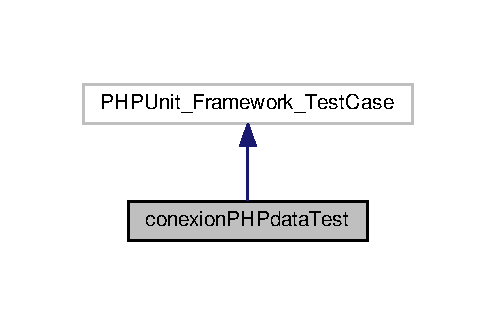
\includegraphics[width=238pt]{de/d1e/classconexionPHPdataTest__inherit__graph}
\end{center}
\end{figure}


Diagrama de colaboración para conexion\-P\-H\-Pdata\-Test\-:\nopagebreak
\begin{figure}[H]
\begin{center}
\leavevmode
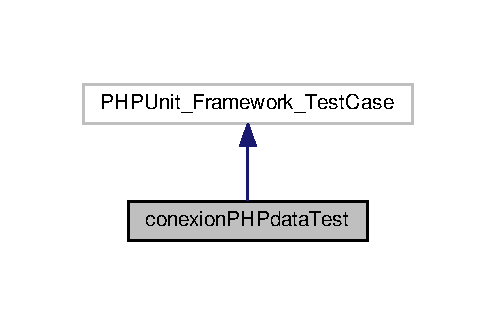
\includegraphics[width=238pt]{d6/d19/classconexionPHPdataTest__coll__graph}
\end{center}
\end{figure}
\subsection*{Métodos públicos}
\begin{DoxyCompactItemize}
\item 
\hyperlink{classconexionPHPdataTest_ab65520d413ff65609ac54582335c7d87}{test\-\_\-conexion\-Establecida} ()
\item 
\hyperlink{classconexionPHPdataTest_ae53ec32ca0ddcf9a3d07ad1a6bf94211}{text\-\_\-insercion\-Correcta} ()
\end{DoxyCompactItemize}


\subsection{Documentación de las funciones miembro}
\hypertarget{classconexionPHPdataTest_ab65520d413ff65609ac54582335c7d87}{\index{conexion\-P\-H\-Pdata\-Test@{conexion\-P\-H\-Pdata\-Test}!test\-\_\-conexion\-Establecida@{test\-\_\-conexion\-Establecida}}
\index{test\-\_\-conexion\-Establecida@{test\-\_\-conexion\-Establecida}!conexionPHPdataTest@{conexion\-P\-H\-Pdata\-Test}}
\subsubsection[{test\-\_\-conexion\-Establecida}]{\setlength{\rightskip}{0pt plus 5cm}conexion\-P\-H\-Pdata\-Test\-::test\-\_\-conexion\-Establecida (
\begin{DoxyParamCaption}
{}
\end{DoxyParamCaption}
)}}\label{classconexionPHPdataTest_ab65520d413ff65609ac54582335c7d87}
\hypertarget{classconexionPHPdataTest_ae53ec32ca0ddcf9a3d07ad1a6bf94211}{\index{conexion\-P\-H\-Pdata\-Test@{conexion\-P\-H\-Pdata\-Test}!text\-\_\-insercion\-Correcta@{text\-\_\-insercion\-Correcta}}
\index{text\-\_\-insercion\-Correcta@{text\-\_\-insercion\-Correcta}!conexionPHPdataTest@{conexion\-P\-H\-Pdata\-Test}}
\subsubsection[{text\-\_\-insercion\-Correcta}]{\setlength{\rightskip}{0pt plus 5cm}conexion\-P\-H\-Pdata\-Test\-::text\-\_\-insercion\-Correcta (
\begin{DoxyParamCaption}
{}
\end{DoxyParamCaption}
)}}\label{classconexionPHPdataTest_ae53ec32ca0ddcf9a3d07ad1a6bf94211}


La documentación para esta clase fue generada a partir del siguiente fichero\-:\begin{DoxyCompactItemize}
\item 
\hyperlink{conexionPHPdataTest_8php}{conexion\-P\-H\-Pdata\-Test.\-php}\end{DoxyCompactItemize}

\chapter{Documentación de archivos}
\hypertarget{conexionPHPdata_8php}{\section{Referencia del Archivo conexion\-P\-H\-Pdata.\-php}
\label{conexionPHPdata_8php}\index{conexion\-P\-H\-Pdata.\-php@{conexion\-P\-H\-Pdata.\-php}}
}
\subsection*{Clases}
\begin{DoxyCompactItemize}
\item 
class \hyperlink{classconexionPHPdata}{conexion\-P\-H\-Pdata}
\begin{DoxyCompactList}\small\item\em Class que permite la conexion entre App y servidor. \end{DoxyCompactList}\end{DoxyCompactItemize}

\hypertarget{conexionPHPdataTest_8php}{\section{Referencia del Archivo conexion\-P\-H\-Pdata\-Test.\-php}
\label{conexionPHPdataTest_8php}\index{conexion\-P\-H\-Pdata\-Test.\-php@{conexion\-P\-H\-Pdata\-Test.\-php}}
}
\subsection*{Clases}
\begin{DoxyCompactItemize}
\item 
class \hyperlink{classconexionPHPdataTest}{conexion\-P\-H\-Pdata\-Test}
\end{DoxyCompactItemize}

\hypertarget{GetData_8php}{\section{Referencia del Archivo Get\-Data.\-php}
\label{GetData_8php}\index{Get\-Data.\-php@{Get\-Data.\-php}}
}
\subsection*{Funciones}
\begin{DoxyCompactItemize}
\item 
\hyperlink{GetData_8php_a3b9e6dcf22f337e934ad2ee04952e58c}{getdata} ()
\begin{DoxyCompactList}\small\item\em Funcion para enviar datos a la app y los busca en la base de datos. \end{DoxyCompactList}\end{DoxyCompactItemize}


\subsection{Documentación de las funciones}
\hypertarget{GetData_8php_a3b9e6dcf22f337e934ad2ee04952e58c}{\index{Get\-Data.\-php@{Get\-Data.\-php}!getdata@{getdata}}
\index{getdata@{getdata}!GetData.php@{Get\-Data.\-php}}
\subsubsection[{getdata}]{\setlength{\rightskip}{0pt plus 5cm}getdata (
\begin{DoxyParamCaption}
{}
\end{DoxyParamCaption}
)}}\label{GetData_8php_a3b9e6dcf22f337e934ad2ee04952e58c}


Funcion para enviar datos a la app y los busca en la base de datos. 

\begin{DoxyReturn}{Devuelve}
string Devuelve los datos que hay en la base de datos. 
\end{DoxyReturn}

\hypertarget{PutData_8php}{\section{Referencia del Archivo Put\-Data.\-php}
\label{PutData_8php}\index{Put\-Data.\-php@{Put\-Data.\-php}}
}
\subsection*{Variables}
\begin{DoxyCompactItemize}
\item 
\hyperlink{PutData_8php_a6efc15b5a2314dd4b5aaa556a375c6d6}{\$data} = new \hyperlink{classconexionPHPdata}{conexion\-P\-H\-Pdata}()
\end{DoxyCompactItemize}


\subsection{Documentación de las variables}
\hypertarget{PutData_8php_a6efc15b5a2314dd4b5aaa556a375c6d6}{\index{Put\-Data.\-php@{Put\-Data.\-php}!\$data@{\$data}}
\index{\$data@{\$data}!PutData.php@{Put\-Data.\-php}}
\subsubsection[{\$data}]{\setlength{\rightskip}{0pt plus 5cm}\$data = new {\bf conexion\-P\-H\-Pdata}()}}\label{PutData_8php_a6efc15b5a2314dd4b5aaa556a375c6d6}

%--- End generated contents ---

% Index
\newpage
\phantomsection
\addcontentsline{toc}{chapter}{Índice}
\printindex

\end{document}
